\documentclass[conference]{IEEEtran}
\IEEEoverridecommandlockouts
% The preceding line is only needed to identify funding in the first footnote. If that is unneeded, please comment it out.
\usepackage{cite}
\usepackage{amsmath,amssymb,amsfonts}
\usepackage{algorithm,algorithmic}
\usepackage{graphicx}
\usepackage{textcomp}
\usepackage{xcolor}

\usepackage[hypertexnames=false,linktocpage=true]{hyperref}
\hypersetup{colorlinks=true,linkcolor=blue,anchorcolor=blue,citecolor=blue,filecolor=blue,urlcolor=blue,bookmarksnumbered=true,pdfview=FitB}

\usepackage{lipsum} % dummy text

\def\BibTeX{{\rm B\kern-.05em{\sc i\kern-.025em b}\kern-.08em
    T\kern-.1667em\lower.7ex\hbox{E}\kern-.125emX}}
\usepackage{tikz}
\usepackage{expl3}
\usepackage{amsmath, amssymb}
\usepackage{xcolor}
\usetikzlibrary{arrows}

% styles
\tikzset{
    circlenode/.style={
        circle,
        draw,
        minimum width=1.2cm
    },
    lstmarrow/.style={
        -latex,
        color=green
    },
    textnode/.style={
        anchor=west,
        xshift=-0.8cm
    }
}

\begin{document}

\title{Leveraging Deep Learning Methodologies for Protein Secondary Structure Prediction}

\author{
\IEEEauthorblockN{Sai Madhur Mallampalli}
\IEEEauthorblockA{\textit{Graduate Student, Computer Science}\\\textit{School of Science, Engineering and Technology}\\
\textit{Penn State Harrisburg, The Pennsylvania State University}\\
Middletown, PA 17057, United States \\
sbm6433@psu.edu}
\and
\IEEEauthorblockN{Hyuntae Na}
\IEEEauthorblockA{\textit{Associate Professor, Computer Science}\\\textit{School of Science, Engineering and Technology} \\\textit{Penn State Harrisburg, The Pennsylvania State University}\\
 Middletown, PA 17057, United States\\
hzn17@psu.edu}
}

\maketitle

\begin{abstract}
Protein secondary structure prediction (PSSP) is critical for understanding protein interactions and aids in drug discovery. Despite being foundational, traditional statistical techniques can lack the accuracy and efficiency required for complex protein structures. This research investigates how advanced deep learning approaches, notably Bi-directional Long Short-Term Memory (Bi-LSTM) networks, might improve protein secondary structure prediction. The study seeks to considerably improve the predictive accuracy of secondary structure prediction from amino acid primary sequences by implementing these approaches on large protein datasets, such as those obtained from PISCES. \end{abstract}

\begin{IEEEkeywords}
Protein Secondary Structure Prediction, BiLSTM, Deep Learning, Data Preprocessing and Visualization
\end{IEEEkeywords}

\section{Introduction}

Proteins are essential components of our bodies and are typically classified into four distinct categories. Protein structures are composed of amino acids that are linked with peptide bonds. The primary structure refers to the way the amino acids are sequenced. The secondary structure is formed by the dihedral angles that surround peptide bonds. The tertiary structure refers to the protein folds. Quaternary structure is produced when folded polypeptide molecules bind to the functional proteins. 
In molecular biology, knowledge of protein secondary structure is essential for designing medications and modeling genetic processes. Alpha-helices, beta-sheets, and random coils are examples of secondary structures in proteins that are essential for determining a protein's three-dimensional conformation, which in turn dictates interactions and functionality. Originally, applying statistical techniques derived from empirical data, the Chou-Fasman \cite{choufasman} and GOR \cite{gor} algorithms have been crucial in predicting these structures. Using information theory and Bayesian statistics, the GOR technique \cite{gor} estimates the probability of secondary structures based on surrounding amino acid characteristics at each place in a protein sequence.
However, these traditional methods often struggle to meet the high accuracy demands posed by increasing protein complexity and larger datasets. With the advent of deep learning, and the usage of Recurrent Neural Networks (RNNs)\cite{redmlp} and Convolutional Neural Networks (CNNs)\cite{cnn} in the secondary structure prediction has shown significant advancements in numerous bioinformatics applications, including protein secondary structure prediction. This paper explores the applications of Bi-LSTM (Bi-directional Long Short-Term Memory) network, a kind of recurrent neural network that processes data points from both past and future states, enhancing learning dynamics and prediction accuracy.   

The methodology leverages comprehensive datasets, culled through PISCES\cite{piscesog}, to train and evaluate the Bi-LSTM model and the objective is to demonstrate that these models significantly outperform traditional statistical methods in predicting protein secondary structures, offering both higher accuracy and computational efficiency. These advancements have implications beyond academia, potentially accelerating the development of new therapeutics and enhancing our understanding of genetic functions. 

\section{Literature Review}

The initial approaches to PSSP were based on statistical methods, leveraging the observation that certain amino acids were more likely to be found in certain kinds of secondary structures. The Chou-Fasman method as reviewed by Wolfgang Kabsch and Christian Sander\cite{predprowolf} is a classic example, using propensities of amino acids to predict secondary structure with a 56\% accuracy. The introduction of machine learning algorithms, including SVMs and early neural networks, marked a significant improvement as they leveraged sequence profiles and sometimes structural information from known protein structures, pushing accuracy rates to 73\%-77\% through SVM and neural networks by Ward JJ, McGuffin LJ, Buxton BF, Jones DT\cite{svmsec}.

With the advent of deep learning, CNNs became popular for their ability to capture local patterns along the sequence. Zhou J and Olga G,\cite{gsndeep} present a new approach for PSSP, using a supervised generative stochastic network (GSN), they incorporated a Markov chain that samples from a conditional distribution of outputs based on inputs by employing a position specific scoring matrices for capturing evolutionary information and binary vectors for encoding amino acid sequences. The convolutional architecture allows the model to process the high-dimensional space of protein sequences effectively, using both local and global information and it achieved an accuracy of 66.4\%

Models like DeepCNF (Deep Convolutional Neural Fields) by Wang, S., Peng, J., Ma, J. et al. \cite{deepcnf} further improved accuracy by integrating sequence features with conditional random fields to capture both complex sequence-structure relationships and interdependencies between adjacent secondary structure labels, achieving accuracies above 80\% for Q3 and 72\% for Q8.

Ahmadi et al.\cite{eonn} focused on enhancing the accuracy of predicting protein secondary structures using evolutionary optimized neural network (EONN) and evolutionary optimized support vector machine (EOSVM) models, incorporating algorithms like genetic algorithm (GA), differential evolution (DE), and particle swarm optimization (PSO). They encoded the input features and integrated evolutionary algorithms coupled with a sliding window size to handle the sequence predictions by achieving accuracy upto 78.83\%. Lyu et al. \cite{redmlp} proposed a reductive model that combines multilayer perceptrons with bidirectional gated recurrent units and hidden markov model profiles to capture information from CB513 dataset for predictions resulting in an increase in accuracy by achieving Q3 accuracy of 83.32\% and Q8 accuracy of 70.51\%. Tamzid et al. \cite{gnn} delve into the usage of Graph Neural Networks for PSSP with an intense focus on graph construction, node embeddings, and the use of SVM for classification through the usage of orthogonal encoding and padding the amino acid sequences on both ends to accommodate the window size and achieved an accuracy of 76.89\%. Hu et al. \cite{bils} incorporated five types of protein features including physio-chemical properties, position specific substitution matrices (PSSM) scores, PSSM count, hidden Markov model (HMM) sequence profiles, and word embedding for amino acid encoding and proposed an ensemble algorithm on BiLSTM to combine multiple sub models with each sub model solving a processing subproblem for each feature with an accuracy of 84.3\% .\cite{litrev65} Yang et. al, approaches have achieved accuracy (about 84\%) that is close to the theoretical limit (88\%) in the Deep Learning domain, and similarly as given by Dewi Pramudi et al. \cite{prepro}, AlphaFold has disrupted the way protein structure prediction by achieving accuracies upto 90\% and pushing the envelope higher.

\section{Methods}

The methodology employed in this project involved extensive data pre-processing and exploratory data analysis on datasets culled through PISCES\cite{pisces}\cite{pisces2} and CB513\cite{cb513} before integrating it with a Bidirectional LSTM Model for the secondary structure prediction from the primary sequence of the amino acids.


\subsection{Data Preprocessing and Visualization}
Multiple datasets containing protein structures with varied sequence identity and resolution cutoffs were preprocessed to gauge the distribution of data and understand the scope and nuances of the subproblems that define the secondary structure predictions. These datasets were imported from CSV files sought through Github repositories \cite{pisces}\cite{pisces2} that used PISCES server to cull data suitable for predictive analysis. The datasets from 2022 contained protein structures filtered at 25\% and 30\% sequence identity and 2.0 and 2.5 Angstrom resolution cutoffs. The inclusion of an archival dataset from 2018 aided in the comparison of the distribution of data. A curated version of a mid-2022 dataset where duplicate entries based on primary sequence identity were removed, retaining only the first occurrence to enhance the training mechanism. The features included features like pdb, primary sequence(seq), and secondary sequence in sst8 and sst3 classifications, length of the sequences named len\_x, nonstdaa which checks if the amino acid is standard or redundant, and irrelevant features like rfac, freerfac and resol as they deal with 3D diffraction. Hence, feature extraction was performed by selecting seq and sst3 as they are the only two features that are required for the classification task.

\begin{figure}[hbtp]
\centerline{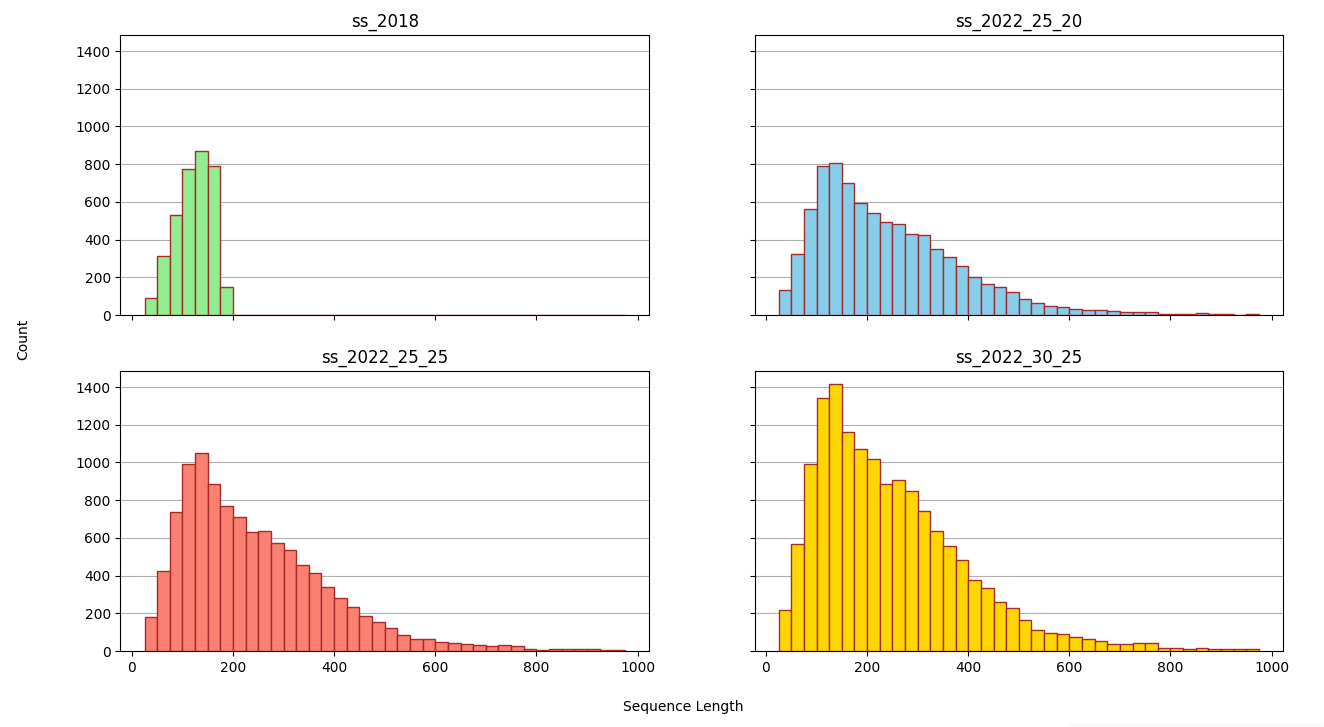
\includegraphics[width=\linewidth]{figs/seqlength.png}}
\caption{
Sequence distribution across datasets based on length.
} 
\label{seqlength}
\end{figure}

\begin{figure}[hbtp]
\centerline{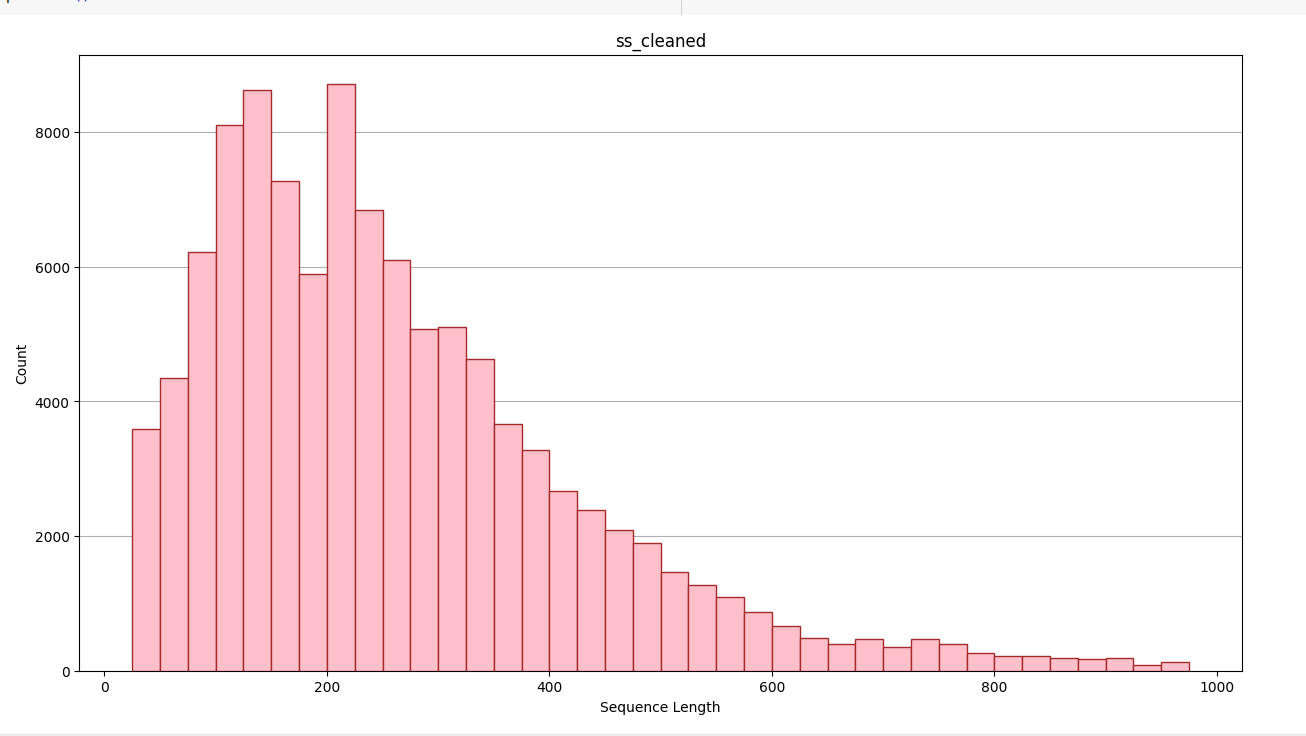
\includegraphics[width=\linewidth]{figs/seqlengthcleaned.png}}
\caption{
Sequence distribution in curated dataset based on length.
} 
\label{seqlengthcleaned}
\end{figure}
The above Figures~\ref{seqlength} and ~\ref{seqlengthcleaned} show the distribution of primary sequences on all the datasets and it is clear that majority of the sequences are between the length 40 - 300 across all data sets.

\subsubsection{Q3 vs Q8}
\begin{figure}[hbtp]
\centerline{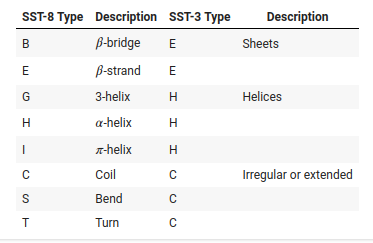
\includegraphics[width=\linewidth]{figs/sst.png}}
\caption{
Secondary Structure Classification
} 
\label{sst}
\end{figure}

Figure~\ref{sst} illustrates how the secondary structure is divided into two types. SST-8, which categorizes into eight specific types, and SST-3, which groups these into three broader categories. In SST-8, the types include: $\beta$-bridge (B), $\beta$-strand (E), 3-helix (G), $\alpha$-helix (H), $\pi$-helix (I), Coil (C), Bend (S), and Turn (T). The SST-3 system simplifies these into Sheets (E), encompassing both $\beta$-strands and $\beta$-bridges; Helices (H), which include $\alpha$-helices, $\pi$-helices, and 3-helices; and Irregular or extended structures (C) such as coils, bends, and turns.

\begin{figure}[hbtp]
\centerline{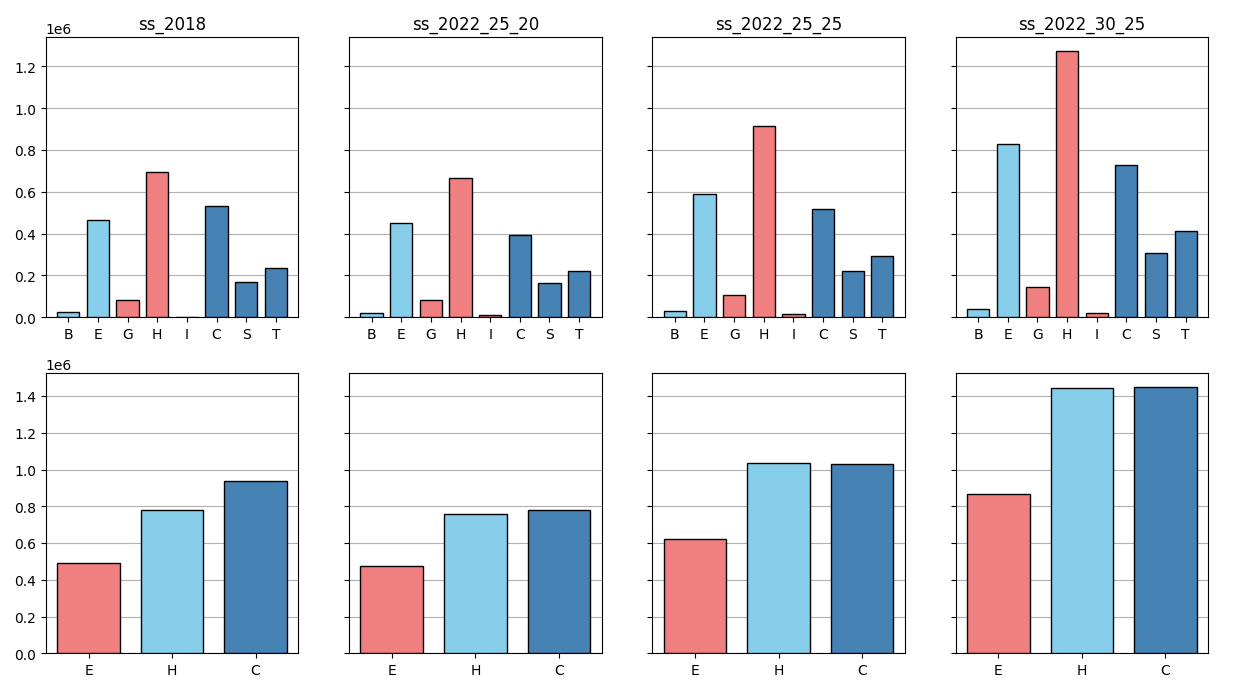
\includegraphics[width=\linewidth]{figs/sst3-8.png}}
\caption{
Secondary Structure distribution among the datasets for testing} 
\label{sst3-8}
\end{figure}

\begin{figure}[hbtp]
\centerline{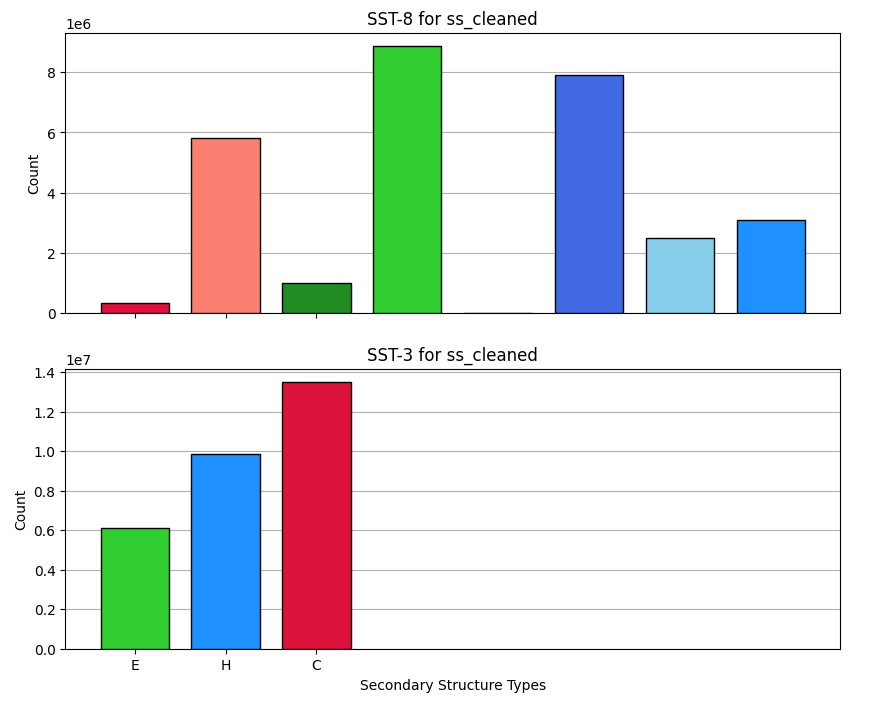
\includegraphics[width=\linewidth]{figs/sst3-8-cleaned.png}}
\caption{
Secondary Structure distribution in the curated dataset for training and validation
} 
\label{sst3-8-cleaned}
\end{figure}
It was observed that Figures~\ref{sst3-8} and ~\ref{sst3-8-cleaned} show the distribution of secondary structure labels on all the datasets and it is evident that the frequency of C and H is higher than E. 

\subsubsection{Data Preparation for Training}
We subset protein sequence data to prepare distinct training, validation, and testing sets, essential for the robust evaluation of predictive models. Sequences were filtered to include only those within a specified length range 40 - 300, enhancing the focus on sequences of relevant sizes for structural prediction and removing outliers. The data underwent further partitioning to create non-overlapping training and validation sets, with additional steps taken to remove internal duplicates within the validation set to maintain data integrity and prevent overfitting.
The primary sequences were transformed into k-mers similar to \cite{kmer} which is an incorporation of n-gram methodology that is utilized in natural language processing tasks to transform sequences to subsequences of specific length k. This technique was followed by the capturing of local sequence features, tokenizing them and encoding them as integers with substantial padding to the specified length to ensure consistency and suitability of data before being fed into the model. Subsequently, the target secondary structures were encoded using the character-level tokenizer that maps each unique structural character to a unique integer and then padded to the same fixed length as the sequence data and then perform one hot encoding on vectors for preparation.
\subsection{Model - Training and Testing}
A Bi-LSTM model was built to implement the prediction and decoding of the secondary structure from the one-hot encoded primary sequence. Bi-LSTM was employed to construct the model as LSTM captures the long-range dependencies within the sequences as the understanding of the entire sequence is crucial in this task as the interaction between the surrounding amino acids can influence the secondary structure. The bidirectionality allowed the model to capture the context from both ends of the sequence providing an inherent well-rounded process that does not overlook integral aspects during the training, validation and testing. 
\ExplSyntaxOn

% number of time steps
\int_new:N \l_step_int
\int_set:Nn \l_step_int {3}

% x spacing and y spacing
\fp_new:N \l_x_space_fp
\fp_set:Nn \l_x_space_fp {1.675}
\fp_new:N \l_y_space_fp
\fp_set:Nn \l_y_space_fp {2}

% LSTM time step offset function
\cs_set:Npn \get_lstm_time:n #1 {
    \int_set:Nn \l_tmpa_int {#1 - 2}
    \int_compare:nNnTF {\l_tmpa_int} = {0} {
        % expands to nothing if the time step is 0
    }{
        \int_compare:nNnTF {\l_tmpa_int} > {0} {
            % show plus sign if greater than 0
            +\int_use:N \l_tmpa_int
        } {
            \int_use:N \l_tmpa_int
        }
    }
}

% LSTM input/output node function
\cs_set:Npn \get_lstm_io:nn #1#2 {
    $
    % add ellipsis
    \int_compare:nNnT {#2} = {1} {
        \cdots
    }
    #1 \c_math_subscript_token {t \get_lstm_time:n {#2}}
    % add ellipsis
    \int_compare:nNnT {#2} = {\l_step_int} {
        \cdots
    }
    $
}

\newcommand{\drawlstm}{
    % append nodes
    \int_step_inline:nn {\l_step_int} {
        % outputs
        \node (o##1) at (\fp_eval:n {##1 * \l_x_space_fp}, 0.0) 
        {\get_lstm_io:nn {y} {##1}};
        % backward layer
        \node[circlenode] (b##1) 
        at (\fp_eval:n {##1 * \l_x_space_fp}, \fp_eval:n {-1 * \l_y_space_fp}) 
        {$\overleftarrow{h\c_math_subscript_token {t \get_lstm_time:n {##1}}}$};
        % forward layer
        \node[circlenode] (f##1) 
        at (\fp_eval:n {##1 * \l_x_space_fp}, \fp_eval:n {-2 * \l_y_space_fp}) 
        {$\overrightarrow{h\c_math_subscript_token {t \get_lstm_time:n {##1}}}$};
        % inputs
        \node (i##1) at (\fp_eval:n {##1 * \l_x_space_fp}, \fp_eval:n {-3 * \l_y_space_fp}) 
        {\get_lstm_io:nn {x} {##1}};
    }
    % draw arrows
    \int_step_inline:nn {\l_step_int - 1} {
        \draw[lstmarrow] (b\int_eval:n {##1 + 1})--(b##1);
        \draw[lstmarrow] (f##1)--(f\int_eval:n {##1 + 1});
    }
    \int_step_inline:nn {\l_step_int} {
        % modify bend left value, if necessary
        \path[lstmarrow] (i##1) edge[bend~left=50] node {} (b##1);
        % modify bend right value, if necessary
        \path[lstmarrow] (f##1) edge[bend~right=50] node {} (o##1);
        \draw[lstmarrow] (i##1)--(f##1);
        \draw[lstmarrow] (b##1)--(o##1);
    }
    % draw edge arrows
    \draw[lstmarrow] (b1)--(0, \fp_eval:n {-1 * \l_y_space_fp});
    \draw[lstmarrow] (\fp_eval:n {(\l_step_int + 1) * \l_x_space_fp}, \fp_eval:n {-1 * \l_y_space_fp})--(b\int_use:N\l_step_int);
    \draw[lstmarrow] (0, \fp_eval:n {-2 * \l_y_space_fp})--(f1);
    \draw[lstmarrow] (f\int_use:N\l_step_int)--(\fp_eval:n {(\l_step_int + 1) * \l_x_space_fp}, \fp_eval:n {-2 * \l_y_space_fp});
    % draw text nodes
    \node[textnode] at (\fp_eval:n {-1 * \l_x_space_fp}, 0)
    {Dense~Layer~Outputs};
    \node[textnode] at (\fp_eval:n {-1 * \l_x_space_fp}, \fp_eval:n {-1 * \l_y_space_fp})
    {Backward~Layer};
    \node[textnode] at (\fp_eval:n {-1 * \l_x_space_fp}, \fp_eval:n {-2 * \l_y_space_fp})
    {Forward~Layer};
    \node[textnode] at (\fp_eval:n {-1 * \l_x_space_fp}, \fp_eval:n {-3 * \l_y_space_fp})
    {Embedding~Layer~Inputs};
}


\ExplSyntaxOff
\begin{center}
    \begin{tikzpicture}
        \drawlstm
    \end{tikzpicture}
\end{center}

The model receives the encoded input at each time step and the embedding layer transforms the discrete tokens into continuous vectors that represent the embedded tokens. The Bidirectional layer processes the embedded inputs in both forward and backward directions, generating a sequence of hidden states for each direction at each time step. The time-distributed dense layer applies a dense neural network to each time step independently, converting the LSTM output at each time step into a more refined representation that maps directly to the desired output space through a softmax activation function and a dropout rate of 0.1 \% to prevent overfitting during training. Once the model was built, it was trained based on varied lengths of the sequences. The model was trained on the curated dataset with no duplication and no overlap with the test sets. To decrease the categorical cross-entropy loss between the actual and predicted values, the accuracy was computed for the encoded characters in the input and output sequences and ignoring padding classes combined with an RMSprop optimizer\cite{rmsprop}. 

The model was trained for 10 epochs achieving a training accuracy of 0.8719 and a validation accuracy of 0.8553. The testing was performed mimicking the approach in training by initially generating the k-mers from the primary sequences from the test sets, tokenizing the k-mers by encoding the kmer strings into sequences of integers where each integer represents a token and padding sequences with zeros to maintain uniformity in length. The target secondary structures were tokenized into kmers, padded to match the length of the input sequences and then the encoded target integer sequences were converted into a binary matrix to be employed in categorical cross-entropy loss calculation during model evaluation. The one-hot encoded predictions were transformed back to the original secondary sequences through a reverse mapping function that uses a reverse index dictionary that interprets the model's predictions and compares them to actual sequences and the Q3 accuracy was calculated.

\section{Experiments and Results}
The model was run on different test sets that were described in the data visualization with the Q3 accuracy ranging from 0.65 to 0.72 for the three-state predictions due to the varied limits for each model and the k-mer size as given in \ref{tab1}. The model performs better when the max length is at 400 as it ensures that the outliers are not taken into consideration and a k-mer size of 3 is chosen.

\begin{table}[htbp]
\caption{Performance Evaluation on Test Sets}
\begin{center}
\begin{tabular}{|c|c|c|}
\hline
\textbf{Datasets} & \textbf{\textit{Q3 Accuracy}} & \textbf{\textit{No of Instances}}\\
\hline
ss\_test& 0.65& 6968\\
\hline
ss\_test\_25\_25& 0.68&4923\\
\hline
ss\_test\_25\_20& 0.72&3774\\
\hline
ss\_test\_2018& 0.69&4058\\
\hline
CB513& 0.71&517\\
\hline
\end{tabular}
\label{tab1}
\end{center}
\end{table}

\begin{figure}[hbtp]
\centerline{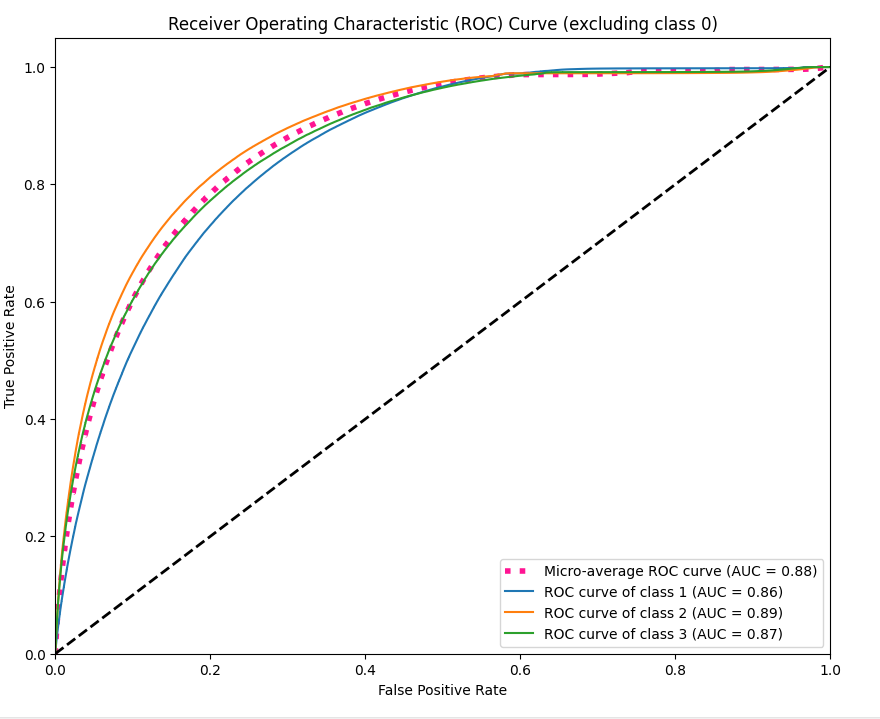
\includegraphics[width=\linewidth]{figs/roc.png}}
\caption{
AUC-ROC for the model} 
\label{roc}
\end{figure}

As shown in \ref{roc}, the AUC is at an average of 0.88 which indicates a good metric for the model.

\section{Conclusions and Future Scope}

The aim of the paper was to explore and understand the dynamics between primary sequence and the three-state secondary structure of protens and demonstrate the efficacy of Bi-directional Long Short-Term Memory (Bi-LSTM) networks in modelling protein secondary structure prediction (PSSP).Using huge datasets combined with data preprocessing and visualization approaches led to a significant increase in accuracy for the BiLSTM model over conventional statistical methods. The model's capacity to examine the underlying intricacies of the protein sequences by utilizing data points at both ends of the k-mer window guaranteed that the complicated relationships are not overlooked. Usage of non-zero classes for training and testing ensured that padded characters do not cloud the model. The future scope in this research domain could include expanding the methodology to eight-state prediction using embedding techniques like orthogonal encoding and interweaving mechanisms like Attention and Transformer with various deep learning techniques like a fusion of BiLSTMs with GNNs that will substantially increase the accuracy of PSSP and eventually aid in 3D modelling of protein structures.
\section*{Acknowledgment}

This document is prepared by referencing Zobel's book~\cite{Zobel14} and wikibook~\cite{wikibook}.

\begin{thebibliography}{00}
\bibitem{choufasman} Chou, Peter Y. and Fasman, Gerald D. Prediction of protein conformation, Biochemistry Vol 13, \url{https://doi.org/10.1021/bi00699a002}
\bibitem{gor}Jean Garnier, Jean-François Gibrat, Barry Robson,
[32] GOR method for predicting protein secondary structure from amino acid sequence, Methods in Enzymology, Academic Press, Volume 266, 1996,ISSN 0076-6879,ISBN 9780121821678,
\url{https://doi.org/10.1016/S0076-6879(96)66034-0}
\bibitem{redmlp} Lyu Z, Wang Z, Luo F, Shuai J, Huang Y. Protein Secondary Structure Prediction With a Reductive Deep Learning Method. Front Bioeng Biotechnol. 2021 Jun 15;9:687426. doi: 10.3389/fbioe.2021.687426. PMID: 34211967; PMCID: PMC8240957.
\bibitem{cnn} Jinyong Cheng, Yihui Liu, Yuming Ma,
Protein secondary structure prediction based on integration of CNN and LSTM model,Journal of Visual Communication and Image Representation, Volume 71, 2020, 102844, ISSN 1047-3203,
\url{https://doi.org/10.1016/j.jvcir.2020.102844.}
\bibitem{piscesog}\url{https://dunbrack.fccc.edu/pisces/}
\bibitem{predprowolf} Wolfgang Kabsch and Christian Sander {\it How good are predictions of protein secondary structure?}, Volume 155, number 2, May 1983 \url{https://febs.onlinelibrary.wiley.com/doi/epdf/10.1016/0014-5793%2882%2980597-8}
\bibitem{svmsec} Ward JJ, McGuffin LJ, Buxton BF, Jones DT. Secondary structure prediction with support vector machines. Bioinformatics. 2003 Sep 1;19(13):1650-5. doi: 10.1093/bioinformatics/btg223. PMID: 12967961 \url{https://pubmed.ncbi.nlm.nih.gov/12967961/}
\bibitem{gsndeep} Zhou J, Olga G, Deep Supervised and Convolutional Generative Stochastic Network for Protein Secondary Structure Prediction. Proceedings of Machine Learning Research, 2014 \url{https://arxiv.org/pdf/1403.1347}
\bibitem{deepcnf} Wang, S., Peng, J., Ma, J. et al. Protein Secondary Structure Prediction Using Deep Convolutional Neural Fields. Sci Rep 6, 18962 (2016). \url{https://doi.org/10.1038/srep18962}
\bibitem{eonn} Ahmadi Toussi, Cyrus \& Haddadnia, Javad. (2019). Improving Protein secondary structure prediction; the evolutionary optimized classification algorithms. Structural Chemistry. 30. 10.1007/s11224-018-1271-5. 
\bibitem{gnn} T. H. Nahid, F. A. Jui and P. C. Shill, "Protein Secondary Structure Prediction using Graph Neural Network," 2021 5th International Conference on Electrical Information and Communication Technology (EICT), Khulna, Bangladesh, 2021, pp. 1-6, doi: 10.1109/EICT54103.2021.9733590.
\bibitem{bils}Hu, Hailong \& Li, Zhong \& Elofsson, Arne \& Xie, Shangxin. (2019). A Bi-LSTM Based Ensemble Algorithm for Prediction of Protein Secondary Structure. Applied Sciences. 9. 3538. 10.3390/app9173538. 
\bibitem{litrev65} Yang Y, Gao J, Wang J, Heffernan R, Hanson J, Paliwal K, Zhou Y. Sixty-five years of the long march in protein secondary structure prediction: the final stretch? Brief Bioinform. 2018 May 1;19(3):482-494. doi: 10.1093/bib/bbw129. PMID: 28040746; PMCID: PMC5952956.
\bibitem{prepro} Dewi Pramudi Ismi, Reza Pulungan,  Afiahayati,
Deep learning for protein secondary structure prediction: Pre and post-AlphaFold,
Computational and Structural Biotechnology Journal,
Volume 20, 2022, Pages 6271-6286, ISSN 2001-0370,
\url{https://doi.org/10.1016/j.csbj.2022.11.012.}
\bibitem{pisces} \url{https://github.com/zyxue/pdb-secondary-structure}
\bibitem{pisces2} \url{https://github.com/KirkDCO/pdb-secondary-structure-2022}
\bibitem{cb513} Avdagic Z, Purisevic E, Omanovic S, Coralic Z. Artificial Intelligence in Prediction of Secondary Protein Structure Using CB513 Database. Summit Transl Bioinform. 2009 Mar 1;2009:1-5. PMID: 21347158; PMCID: PMC3041573.
\bibitem{kmer}\url{https://www.kaggle.com/code/helmehelmuto/secondary-structure-prediction-with-keras/notebook}
\bibitem{rmsprop} \url{https://medium.com/analytics-vidhya/a-complete-guide-to-adam-and-rmsprop-optimizer-75f4502d83be}
\bibitem{Zobel14} Justin Zobel, {\it Writing for Computer Science}, 3rd ed., Springer, 2014.
\bibitem{wikibook} \url{https://en.wikibooks.org/wiki/LaTeX}
\bibitem{wikibook-alg} \url{https://en.wikibooks.org/wiki/LaTeX/Algorithms}
\end{thebibliography}

\end{document}
